\chapter{Testy}
\label{cha:testy}

Poniżej prezentujemy testy jakie przeprowadzliśmy wraz z ich krótkim opisem oraz niezbędnymi zmianami w kodzie oraz komentarzem odnoszącym się do rezultatów otrzymywanych z w3af. 
\section{XSS}

\begin{enumerate}
\item Opis podatności\\
 Sposób ataku na serwis WWW polegający na osadzeniu w treści atakowanej strony kodu (zazwyczaj JavaScript), który wyświetlony innym użytkownikom może doprowadzić do wykonania przez nich niepożądanych akcji. Skrypt umieszczony w zaatakowanej stronie może obejść niektóre mechanizmy kontroli dostępu do danych użytkownika.

\item Zmiany w kodzie\\
Zmieniliśmy plik calendar view.php. Przeprowadzone zmiany miały na celu ekspozycję jednego z parametrów.

\noindent
\begin{minipage}{\linewidth}
\makebox[\linewidth]{
  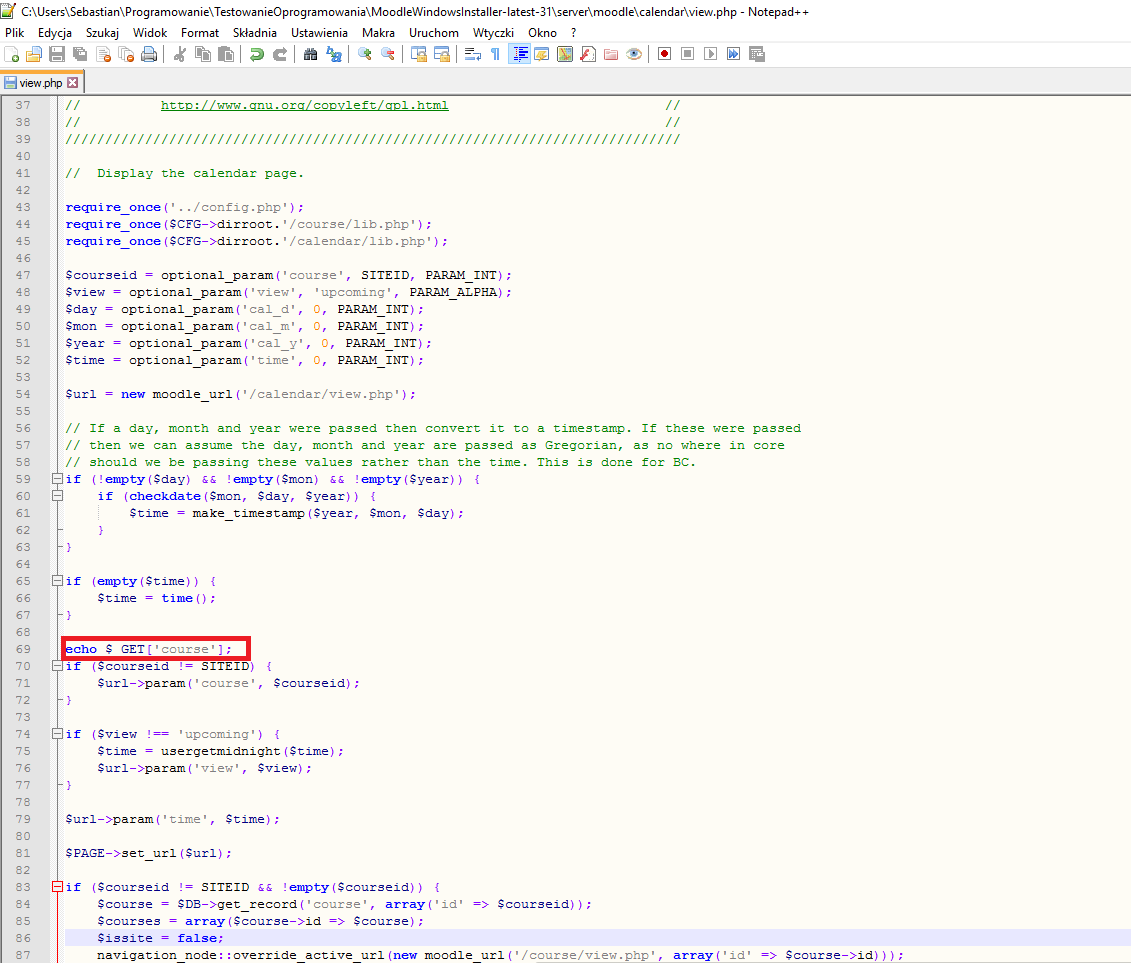
\includegraphics[keepaspectratio=true,scale=0.5]{pictures/xss_error_code_change.png}}
\captionof{figure}{Wyniki W3AF z logów - wykryta podatność}\label{erd}
\end{minipage}
\end{enumerate}

\item Komentarz\\
W3AF znalazł podatność na atak XSS:

\noindent
\begin{minipage}{\linewidth}
\makebox[\linewidth]{
  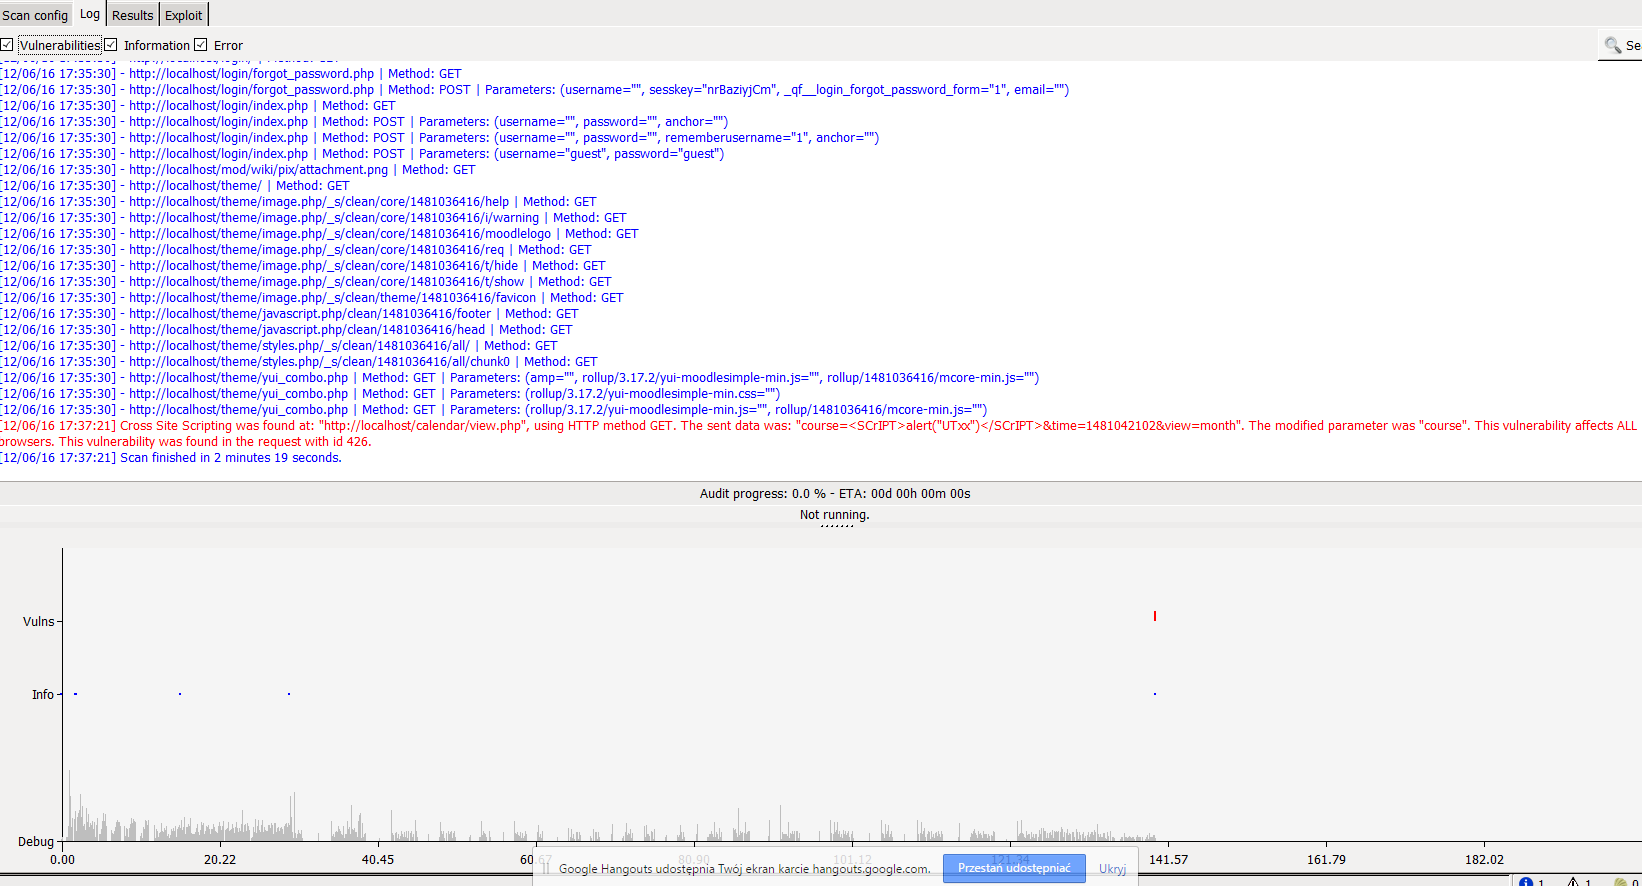
\includegraphics[keepaspectratio=true,scale=0.3]{pictures/xss_log_error.png}}
\captionof{figure}{Wyniki W3AF z logów - wykryta podatność}\label{erd}
\end{minipage}
\end{enumerate}

\noindent
\begin{minipage}{\linewidth}
\makebox[\linewidth]{
  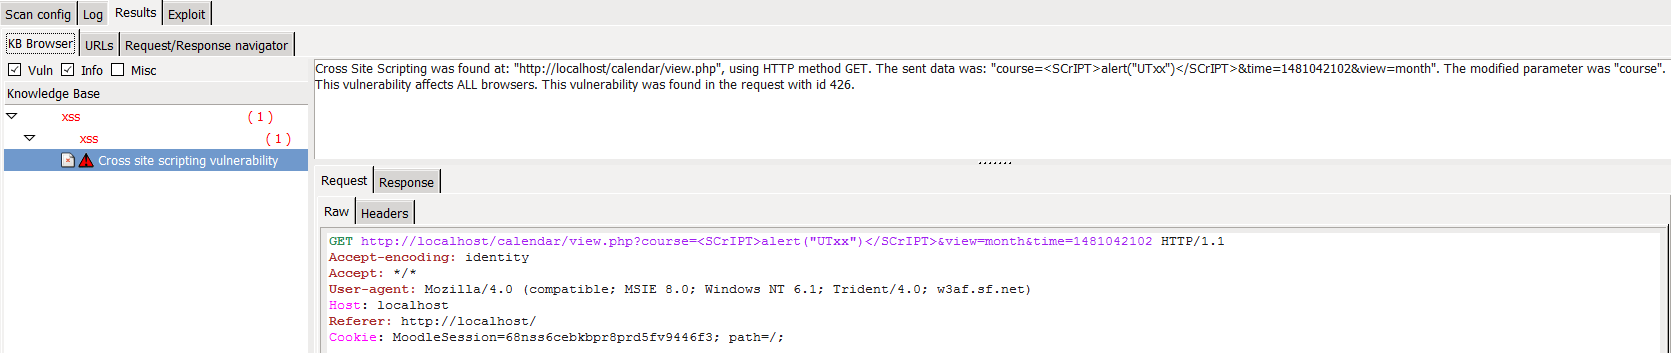
\includegraphics[keepaspectratio=true,scale=0.3]{pictures/xss_results.png}}
\captionof{figure}{Wyniki W3AF z bazy wiedzy na temat xss}\label{erd}
\end{minipage}
\end{enumerate}

%-------------------------------------

\section{SQL injection}
\begin{enumerate}
\item Opis podatności\\
 metoda ataku komputerowego wykorzystująca lukę w zabezpieczeniach aplikacji polegającą na nieodpowiednim filtrowaniu lub niedostatecznym typowaniu danych użytkownika, które to dane są później wykorzystywane przy wykonaniu zapytań (SQL) do bazy danych. Podatne są na nią wszystkie systemy przyjmujące dane od użytkownika i dynamicznie generujące zapytania do bazy danych.
\item Zmiany w kodzie\\
Nie były wymagane w przypadku tej podatności.
\item Komentarz\\
W3AF, a konkretnie plugin blind\_sqli znalazł podatność na CSRF podczas pierwszego uruchomienia testów. Podatne na atak SQL injection są miejsca wpisywania loginu i hasła przez użytkownika.
\noindent
\begin{minipage}{\linewidth}
\makebox[\linewidth]{
  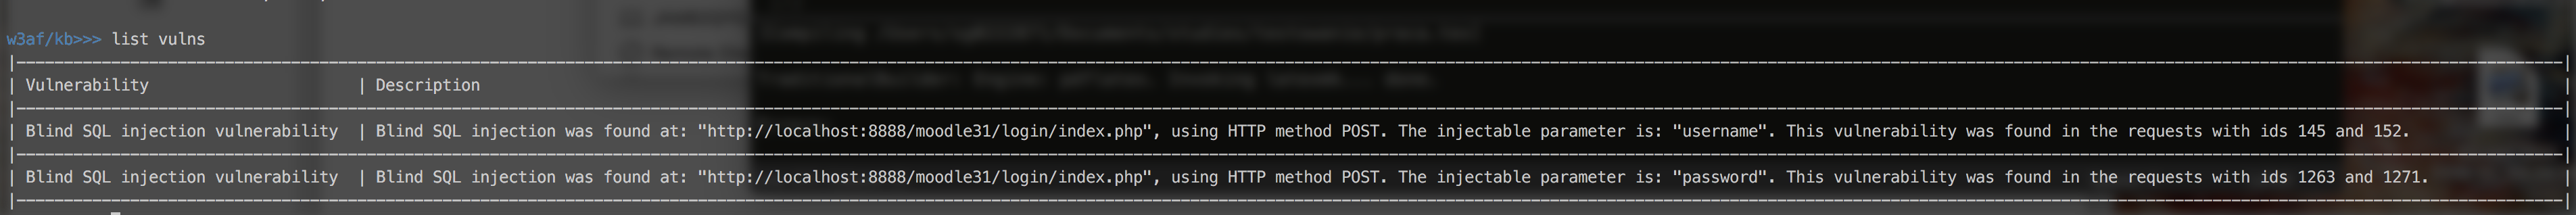
\includegraphics[keepaspectratio=true,scale=0.3]{pictures/sqli.png}}
\captionof{figure}{Wyniki W3AF z bazy wiedzy na temat sql injection}\label{erd}
\end{minipage}
\end{enumerate}

%-------------------------------------

\section{Guessable credentials}
\begin{enumerate}
\item Opis podatności\\
Test ten umożliwia nam sprawdzenie czy aplikacja webowa została nieodpowiedni zabezpieczona przed stworzeniem w niej kont z stosunkowo łatwymi do odgadnięcia hasłami co w konsekwencji może prowadzić do dokonania ataku słownikowego.
\item Zmiany w kodzie\\
Nie były wymagane
\item Komentarz\\
W testowanej przez nas aplikacji okazało się że występują pewne uchybienia, które sprawiły iż test guessable credentials nie został zakończony pozytywnie - Na poniższych screenach widać, że portal Moodle umożliwia stworzenie kont z bardzo trywialnymi hasłami takimi jak null  czy też 5up3rv150r

\noindent
\begin{minipage}{\linewidth}
\makebox[\linewidth]{
  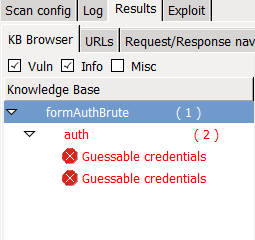
\includegraphics[keepaspectratio=true,scale=0.7]{pictures/guessable_credentials.png}}
\captionof{figure}{Znalezione podatności na guessabe_credentials.}\label{erd}
\end{minipage}

\noindent
\begin{minipage}{\linewidth}
\makebox[\linewidth]{
  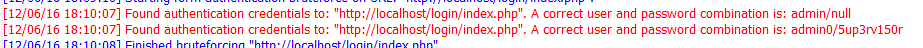
\includegraphics[keepaspectratio=true,scale=0.7]{pictures/guessable_credentials_log.png}}
\captionof{figure}{Log W3AF na temat wykrytych podatności.}\label{erd}
\end{minipage}

\noindent
\begin{minipage}{\linewidth}
\makebox[\linewidth]{
  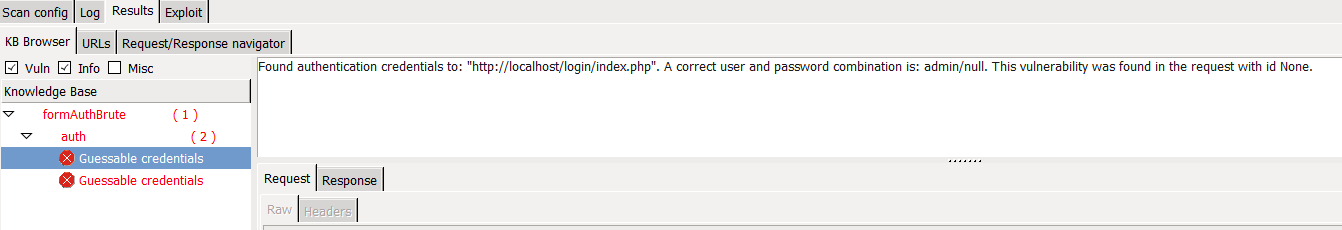
\includegraphics[keepaspectratio=true,scale=0.5]{pictures/guessable_credentials_description.png}}
\captionof{figure}{Opis pierwszej wykrytej podatności}\label{erd}
\end{minipage}

\noindent
\begin{minipage}{\linewidth}
\makebox[\linewidth]{
  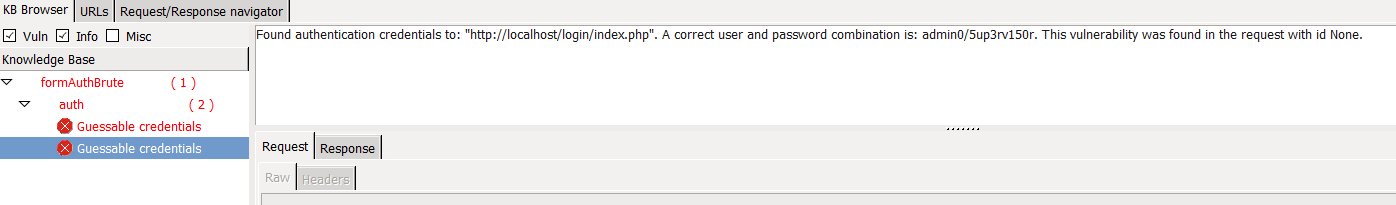
\includegraphics[keepaspectratio=true,scale=0.5]{pictures/guessable_credentials_description2.png}}
\captionof{figure}{Opis drugiej wykrytej podatności}\label{erd}
\end{minipage}
\end{enumerate}


%-------------------------------------

\section{Click-Jacking}
\begin{enumerate}
\item Opis podatności\\
CLick-Jacking to złośliwa technika nakłaniające użytkowników do klikania w inne rzeczy niż oni sami myślą, że klikają.
Może dojść do potencjalnego ujawnienia poufnych inforamcji lub przejęcia kontroli nad ich komputerem, po kliknięciu na pozornie niewinną stronę. Click-jacking przybiera też formę wbudowanego kodu lub skryptu, który może został wywołany bez wiedzy użytkownika.
\item Zmiany w kodzie\\
Nie były wymagane w przypadku tej podatności.
\item Komentarz\\
W3AF podczas pierwszego uruchomienia, bez zmian w kodzie, wykrył podatność aplikacji Moodle na brak zabezpieczeń przed atakami click-jacking. 
\end{enumerate}

\noindent
\begin{minipage}{\linewidth}
\makebox[\linewidth]{
  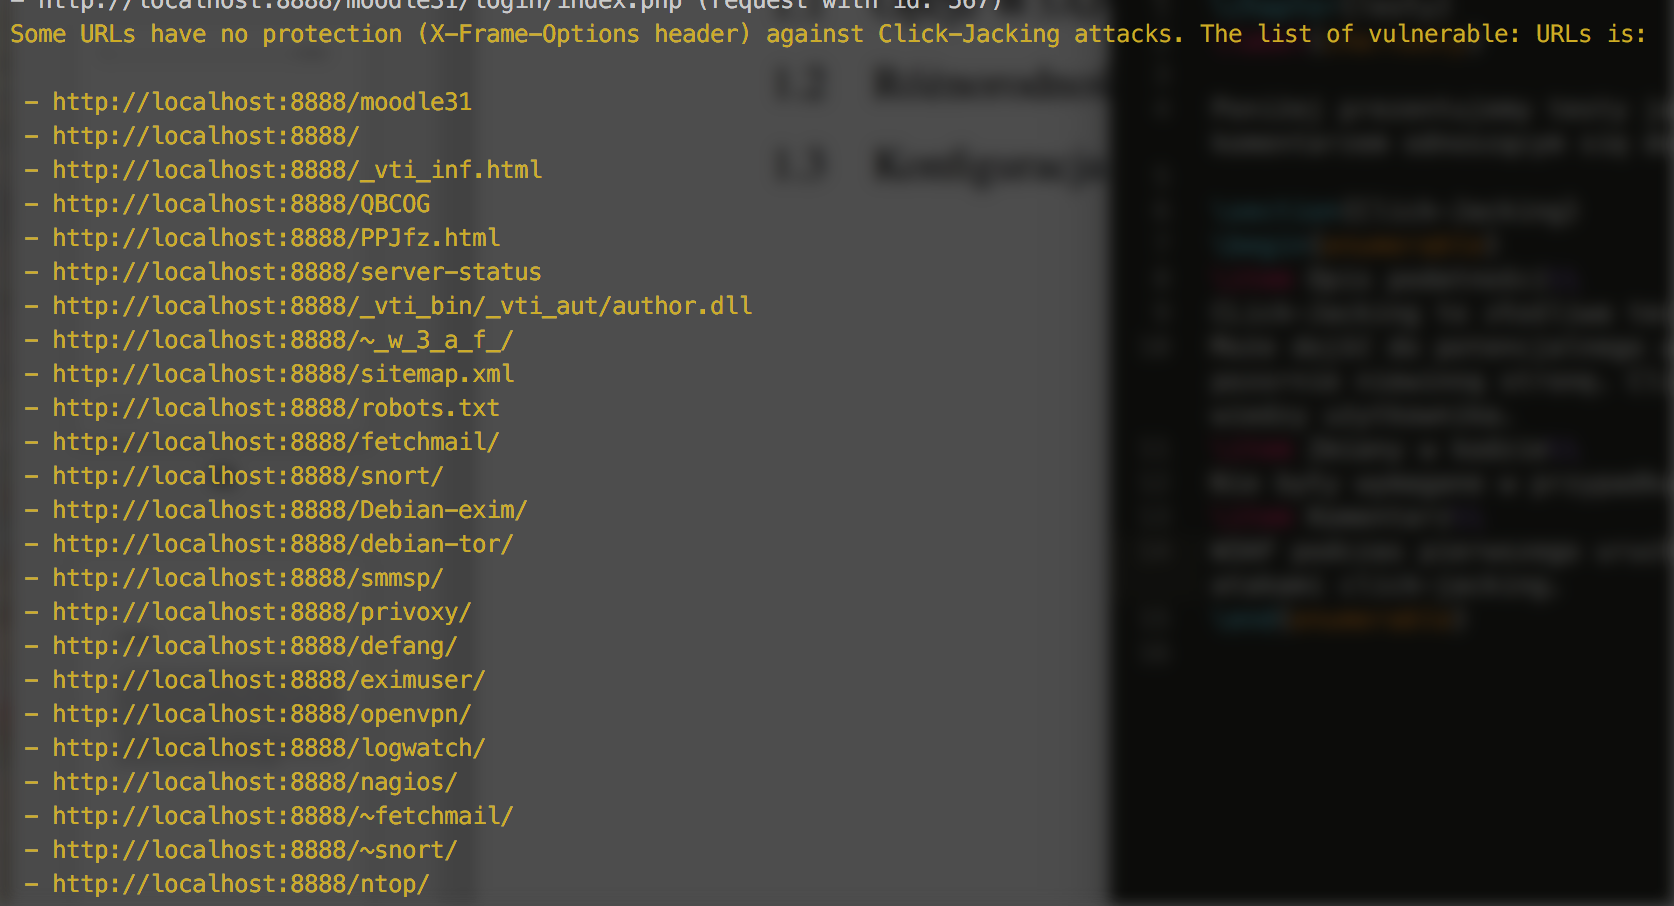
\includegraphics[keepaspectratio=true,scale=0.5]{pictures/clickjacking.png}}
\captionof{figure}{Wyniki W3AF dotyczące clickjackingu}\label{erd}
\end{minipage}

%--------------------------------------

\section{CSRF}
\begin{enumerate}
\item Opis podatności\\
CSRF - metoda ataku na serwis internetowy, która często (m.in. na skutek jednoczesnego wykorzystania) mylona jest z cross-site scripting (XSS) bądź jest uznawana za jej podzbiór. Ofiarami CSRF stają się użytkownicy nieświadomie przesyłający do serwera żądania spreparowane przez osoby o wrogich zamiarach. W przeciwieństwie do XSS, ataki te nie są wymierzone w strony internetowe i nie muszą powodować zmiany ich treści. Celem crackera jest wykorzystanie uprawnień ofiary do wykonania operacji w przeciwnym razie wymagających jej zgody. Błąd typu CSRF dotyczy również serwerów FTP. 
\item Zmiany w kodzie\\
Nie były wymagane w przypadku tej podatności.
\item Komentarz\\
W3AF znalazł podatność na CSRF podczas pierwszego uruchomienia testów bez wprowadzania zmian w kodzie:
\noindent
\begin{minipage}{\linewidth}
\makebox[\linewidth]{
  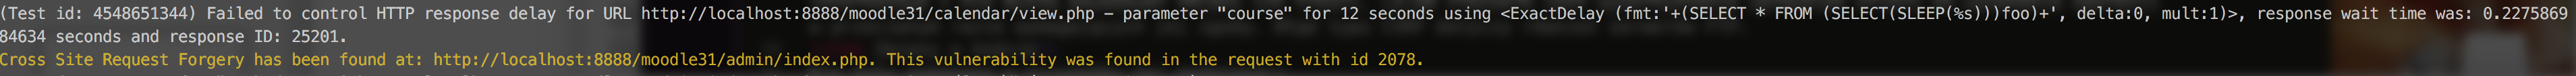
\includegraphics[keepaspectratio=true,scale=0.3]{pictures/csrf.png}}
\captionof{figure}{Wyniki W3AF dotyczące cross site request forgery}\label{erd}
\end{minipage}
\end{enumerate}

\noindent
\begin{minipage}{\linewidth}
\makebox[\linewidth]{
  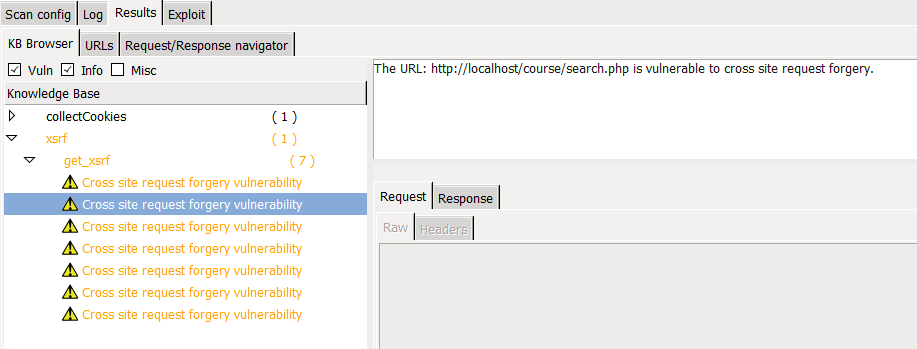
\includegraphics[keepaspectratio=true,scale=0.7]{pictures/csrf_result2.png}}
\captionof{figure}{Wyniki W3AF dotyczące cross site request forgery (GUI)}\label{erd}
\end{minipage}
\end{enumerate}

%--------------------------------------

\section{Security misconfiguration}
\begin{enumerate}
\item Opis podatności\\
Plugin w w3af zajdujący sie w sekcji discovery o nazwie domain_dot, który wynajduje błędna konfigurację przez wysyłanie specjalnych zapytań z kropkami w nazwie.  Dla przykładu, jeżeli celem jest http://moodle.pl/ , plugin stworzy zapytanie http://moodle.pl./
\item Zmiany w kodzie\\
Nie były wymagane
\item Komentarz\\
Dzięki niektórym błędnym konfiguracjom, atakujący jest w stanie przeczytać kod źródłowy aplikacji webowych przez punktowe zapytanie. W Moodle testy tej słabości systemu przeszły bezbłędnie, nie ma żadnych błędów co widać na poniższych screenach
\noindent
\begin{minipage}{\linewidth}
\makebox[\linewidth]{
  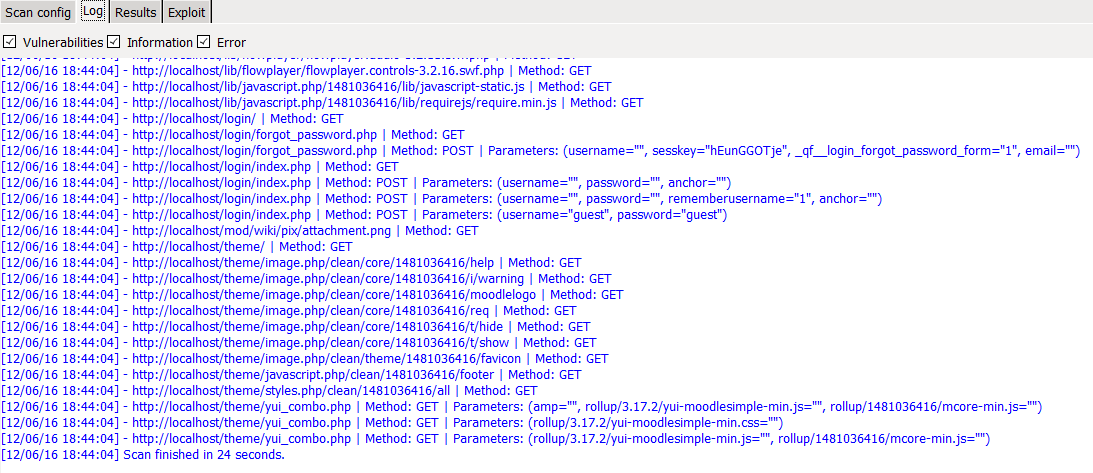
\includegraphics[keepaspectratio=true,scale=0.6]{pictures/security_misconfiguration_log.png}}
\captionof{figure}{Log dotyczący podatności na security misconfiguration}\label{erd}
\end{minipage}

\noindent
\begin{minipage}{\linewidth}
\makebox[\linewidth]{
  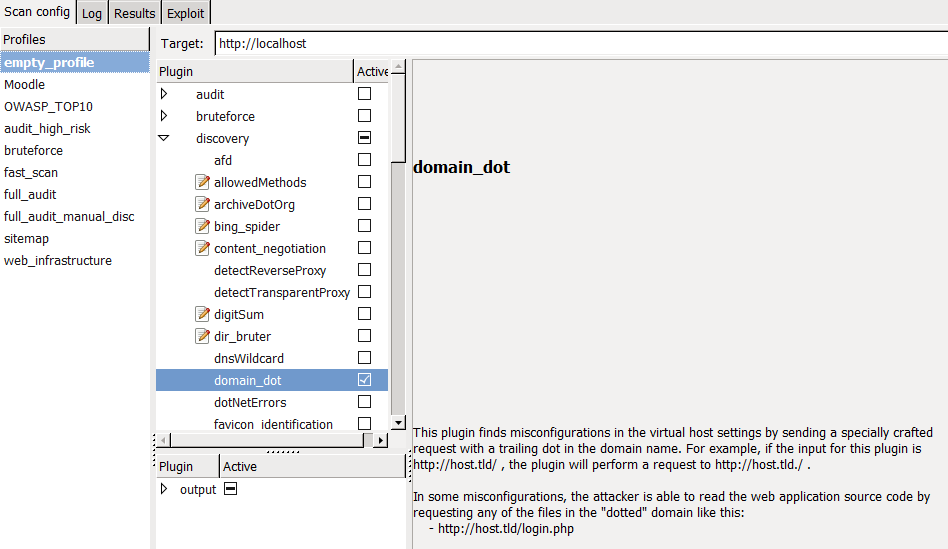
\includegraphics[keepaspectratio=true,scale=0.6]{pictures/security_misconfiguration.png}}
\captionof{figure}{Wykryte podatności na security misconfiguration}\label{erd}
\end{minipage}
\end{enumerate}

\end{enumerate}

